\section{Justering ift. matematisk model af PTS}
\label{ss:regulatorMat}
Som beskrevet i afsnit \ref{ss:ValgReg} er det valgt at implementere to PI-regulatorer.
Der tages udgangspunkt i den matematiske model af systemet, bestående af overføringsfunktionerne
\(G_{tilt,zoh}\) og \(G_{pan,zoh}\), som er diskretiseringer af de kontinuerte overføringsfunktioner.
Der skal findes to sæt koefficienter, \(K_P\) og \(K_I\), et sæt til hver regulator.
For at medtage den væsentligste ulinearitet, dødzonen, i regulatordesignet,
er det valgt at simulere systemet i Simulink.
I Simulink er den diskretiserede overføringsfunktion indsat sammen med en model for dødzonen,
målt eksperimentelt, samt PI-regulatoren. Det simulerede systems blokdiagram er illustreret i figur \ref{fig:simulink1}.
Da modellen indeholder ulineariteter er det valgt at starte med et simpelt gain \(K_P\) på 1,
og med Trial-and-Error metoden prøve sig frem til koefficienterne.
Begge regulatorer gives et parabelinput, og deres performance vurderes
efter deres evne til at følge parablen. Dvs. det er forsøgt at minimere Tracking fejlen.


\begin{figure}[!th]
\centering
\begin{tikzpicture}[auto, node distance=2.6cm,>=latex']
%\begin{tikzpicture}[scale=0.9, every node/.style={scale=0.9}, node distance=2.6cm, =>latex']
\include*{./graphics/simulink1}
\end{tikzpicture}
\caption[Simuleret system]
		{Simuleret system. Tilbagekoblingsblokken angiver, at outputsignalet kvantiseres med et interval på \(q\mathrm{:} \frac{1}{1080}\),
		for at simulere motorens encoder feedback.
		\(D\left(z\right)\) er PI-regulatoren.}
\label{fig:simulink1}
\end{figure}


Med ovenstående metode blev koefficienterne i tabel \ref{tb:pidSimulink} fundet tilfredsstillende.
Koefficienterne i tabel \ref{tb:pidSimulink} benævnes startkoefficienterne, da regulatorjusteringen
ift. det fysiske system starter med disse værdier.
Tracking fejlen er afbildet i figur \ref{fig:pidSim1}, og som det ses af grafen, når den maks. 0,5 \degree{} i simuleringen.

\begin{figure}[h!]
\centering
\begin{tabu}{l|[1.25pt]c|c|c}
      & \(K_P\) & \(K_I\) & \(K_D\)\\\tabucline[1.25pt]{-}
Tilt  & 240 & 85 & -\\\hline%0,248960\\\hline
Pan   & 240 &  100 & -
\end{tabu}
\captionsetup{type=table}
\caption[Regulatorkoefficienter]{Koefficienter fundet vha. simulering.}
\label{tb:pidSimulink} 
\end{figure}

\begin{figure}[h!]
\centering
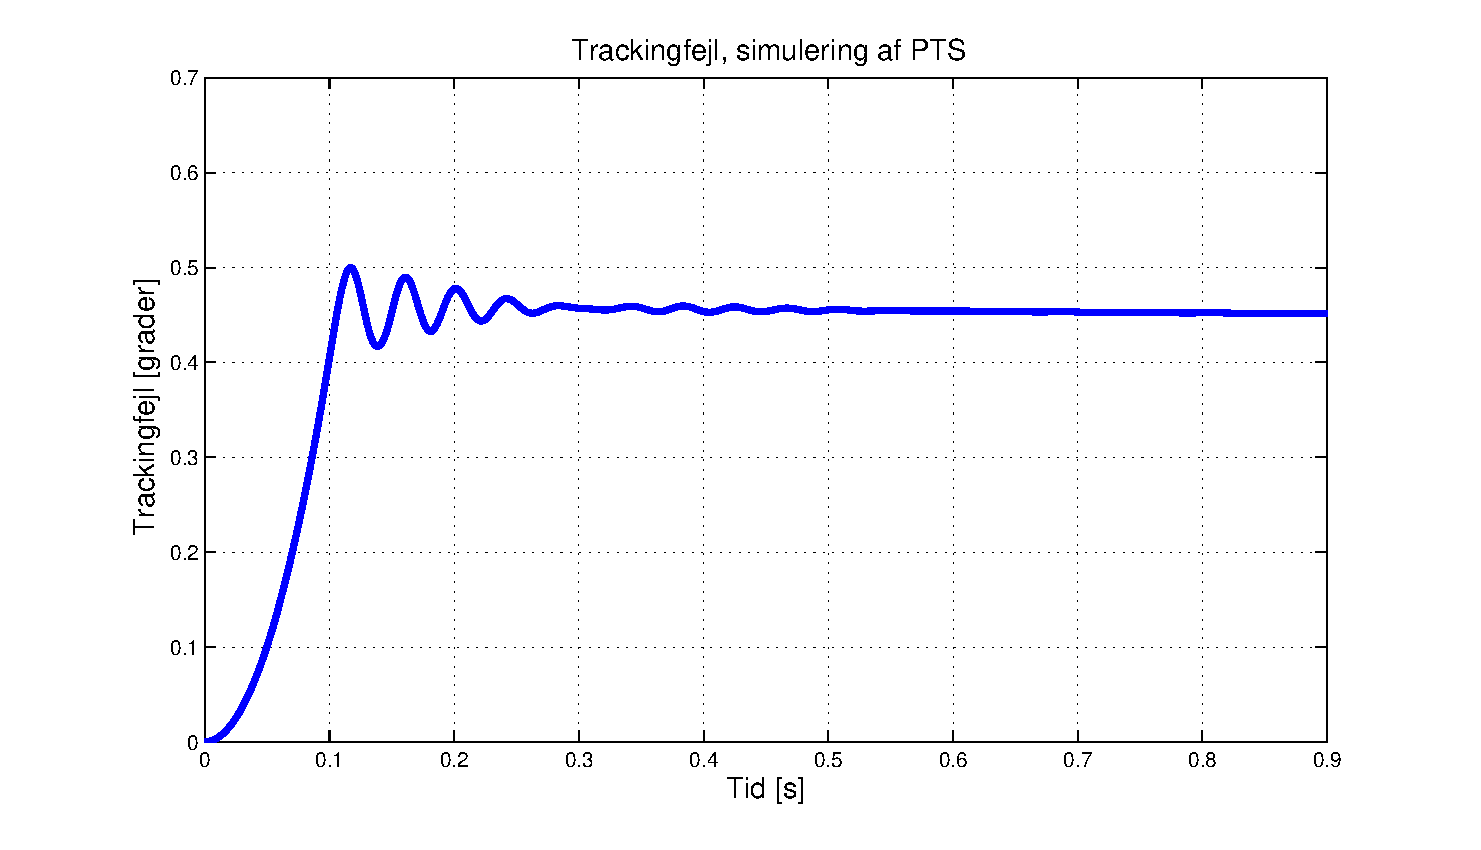
\includegraphics[width=1\textwidth]{./graphics/pidSim1.eps}
\caption[Tracking fejl ved simulering]{Tracking fejl ved simulering af PTS med regulatorkoefficienterne fra tabel \ref{tb:pidSimulink}.} 
\label{fig:pidSim1}
\end{figure}

De to regulatorer er med startkoefficienterne blevet afprøvet i praksis.
Figurer \ref{fig:pidPhys1} viser Pan-fejlsignalet (rød) og Tilt-fejlsignalet (blå)
i forhold til den kontinuerte lerdueparabel fra applikationen.

\begin{figure}[h!]
\centering
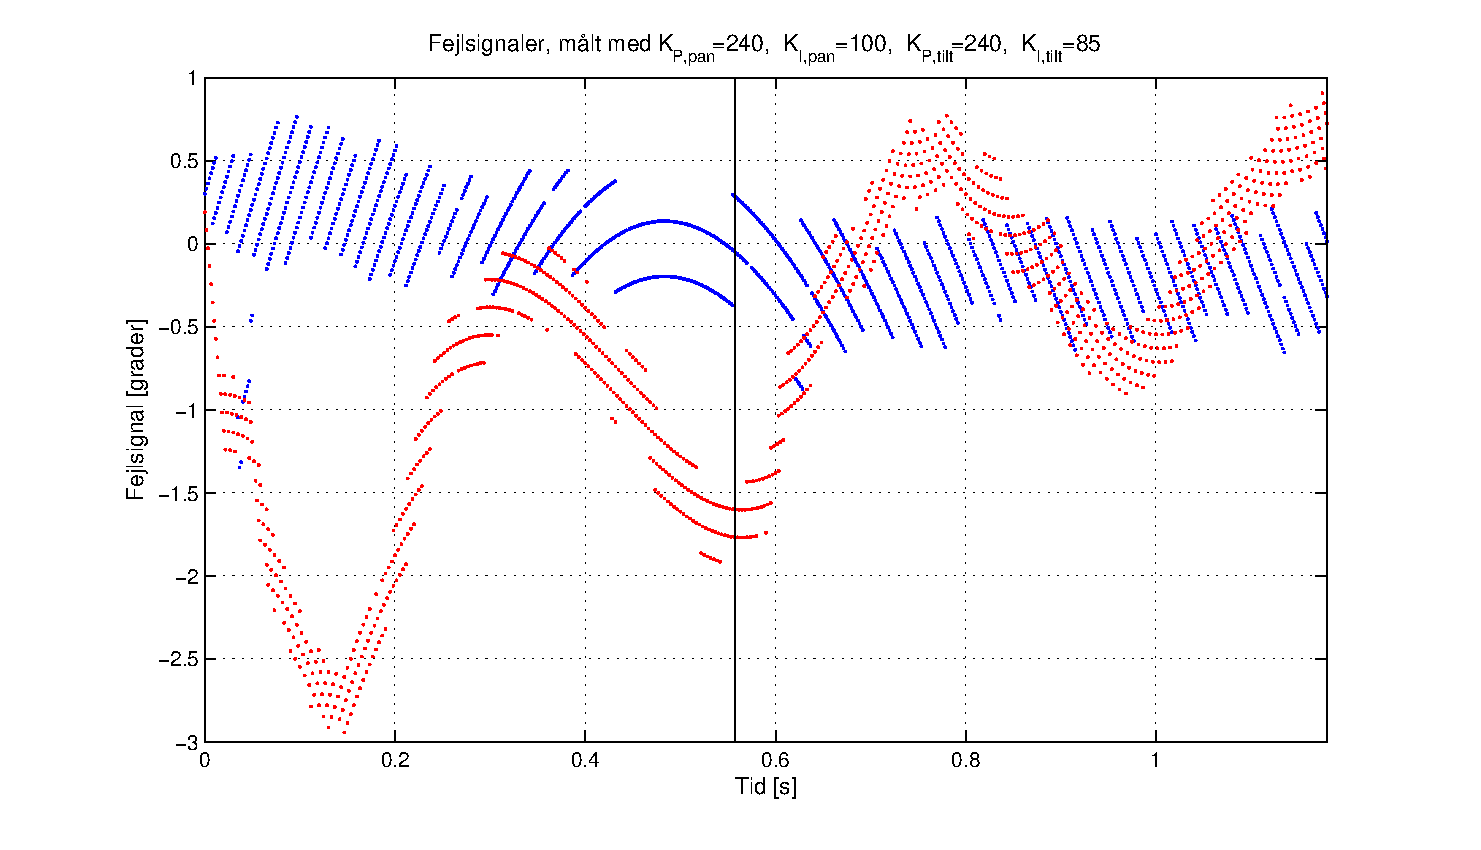
\includegraphics[width=1\textwidth]{./graphics/pidPhys1.eps}
\caption[Fejlsignaler m. startkoefficienter]{Fejlsignaler m. startkoefficienterne fra tabel \ref{tb:pidSimulink}.
	De sorte lodrette streger angiver \(t_s=0,557 \text{ [s]}\).\\
	Pan-fejlsignalet er markeret med prikker, og Tilt-fejlsignalet er markeret med krydser.} 
\label{fig:pidPhys1}
\end{figure}

Som det ses på figur \ref{fig:pidPhys1} giver regulatoren til Tilt et fejlsignal,
der maks. afviger 0,9 \degree{} fra 0.
Pan-fejlen afviger derimod op til 1,8 \degree{}.
Tracking fejlen er altså langt større end kravet på maksimalt 1,02 \degree.
En manuel justering af koefficienterne på især Pan-regulatoren er derfor nødvendig.

\section{Manuel justering ift. fysisk PTS}
Ved at ændre på koefficienterne og analysere fejlgraferne justeres performance 
hen mod det ønskede.

Det vurderes på baggrund af det lave fejlsignal ved Tilt at den i afsnit \ref{ss:regulatorMat} fundne
PI-regulator for Tilt er anvendelig i praksis.

På Pan er der behov for en hurtigere og mere dæmpet reaktion,
og det vurderes derfor, at der på Pan er brug for en PID-regulator.

\subsection{Valg af integratormætning}
Det vælges at sætte integratormætningen til 100 for begge regulatorer, da det vurderes, at der drages
fuld nytte af integratorleddet når ligning \ref{eq:integratorsaturation} 
overholdes.

\begin{equation}
	K_I \cdot Integrator_{Max} > PWM_{Max}
\label{eq:integratorsaturation} 
\end{equation}

\todo[inline,color=Pink,author=Mikkel]{Måske for kvalitativt. Måske må man ikke bare lave sin egen ligning, men jeg har ikke nogne kilde.}

\subsection{Tilføjelse af et D-filter}
Undervejs i den manuelle justering af PID-regulatoren til Pan blev det fundet, at D-leddet ikke udnyttedes til fulde,
og at kravene ikke kunne overholdes med PID-regulatoren som den var.
Det valgtes derfor at tilføje et filter til D-leddet. 
Det betyder at D-leddet nu vægter tidligere ændringer i fejlsignalet. 
Filtret reducerer peaks i det differrentierede fejlsignal, der skyldes Zero Order Hold i upsamplingen (se afsnit \ref{subsec:upsampling}).

Der implementeres et 4. ordens FIR filter. Filtret er designet i MATLAB's grafiske fdatool og gør brug af at Kaiser vindue.
Filtrets step- og frekvensrespons kan ses på figur \ref{fig:d_filter_step} hhv. \ref{fig:d_filter_bode}. 

\begin{figure}[h!]
\centering
\subfloat[Steprespons for det implementerede filter.\label{fig:d_filter_step}]{%
	\hspace*{-0.6cm}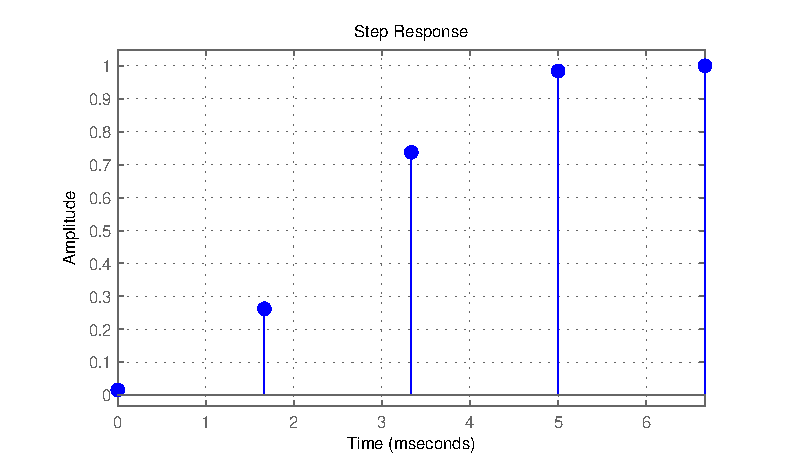
\includegraphics[width=0.57\textwidth]{./graphics/d-filter-step-small}
}
\subfloat[Frekvensrespons for det implementerede filter.\label{fig:d_filter_bode}]{%
	\hspace*{-1.15cm}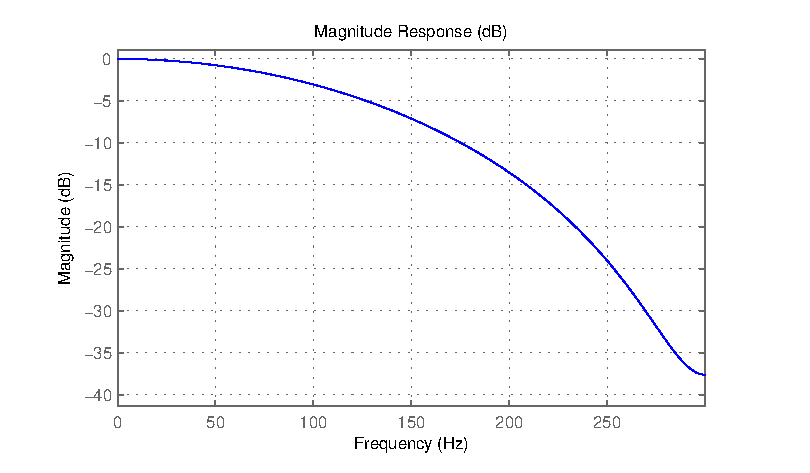
\includegraphics[width=0.57\textwidth]{./graphics/d-filter-bode-small}
	
}
\caption[D-filterets respons]{Dette er ikke en figur tekst. }
\label{fig:d_filter}
\end{figure}

\section{Endelig performance}
Efter adskillige test og finjustering af regulatoren, vurderes det at 
koefficienterne i tabel \ref{tb:PID_final} giver den bedst mulige performance 
for PTS. Denne performance ses i \ref{fig:PID_final}. Det ses at trackingfejlen 
holder sig inden for de 1,02$\degree$  pånær ved et par enkelte samples.

\begin{figure}[h!]
\centering
\begin{tabu}{l|[1.25pt]c|c|c}
      & \(K_P\) & \(K_I\) & \(K_D\)\\\tabucline[1.25pt]{-}
Tilt  & 240 & 85 & -\\\hline
Pan   & 100 & 110 & 3,8
\end{tabu}
\captionsetup{type=table}
\caption[Endelige regulatorkoefficienter]{De endelige regulatorkoefficienter.}
\label{tb:PID_final} 
\end{figure}

\begin{figure}[h!]
\centering
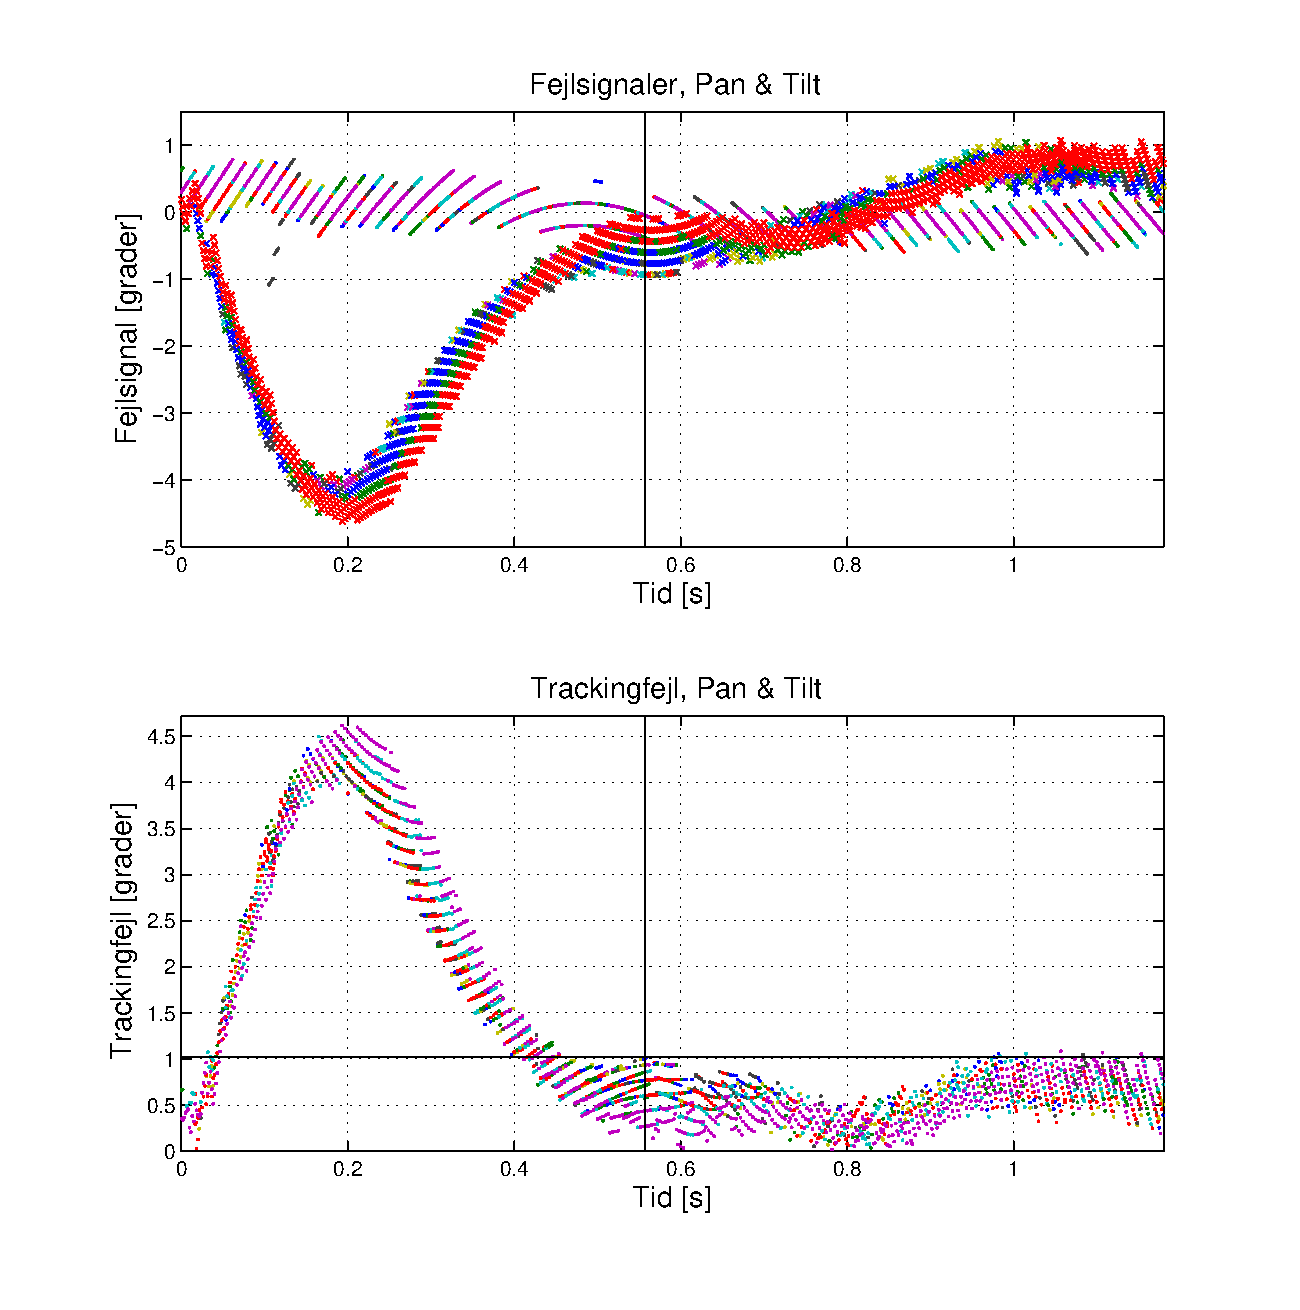
\includegraphics[width=1\textwidth]{./graphics/pidPhys2.eps}
\caption[Endelig performance]{Endelig performance. Fejlsignaler for Pan (krydser) og Tilt (prikker) øverst, Tracking fejl nederst.
Testen er foretaget med koefficienterne fra tabel \ref{tb:PID_final}.} 
\label{fig:PID_final}
\end{figure}
%
%\begin{figure}[h!]
%\centering
%\begin{tabu}{l|[1.25pt]c|c|c}
%      & \(K_P\) & \(K_I\) & \(K_D\)\\\tabucline[1.25pt]{-}
%Tilt  & 49 & 32,5 & 0\\\hline
%Pan   & 80 & 160 & 3,55
%\end{tabu}
%\captionsetup{type=table}
%\caption[Endelige regulatorkoefficienter]{De endelige regulatorkoefficienter.}
%\label{tb:PID_final} 
%\end{figure}
%
%\begin{figure}[h!]
%\centering
%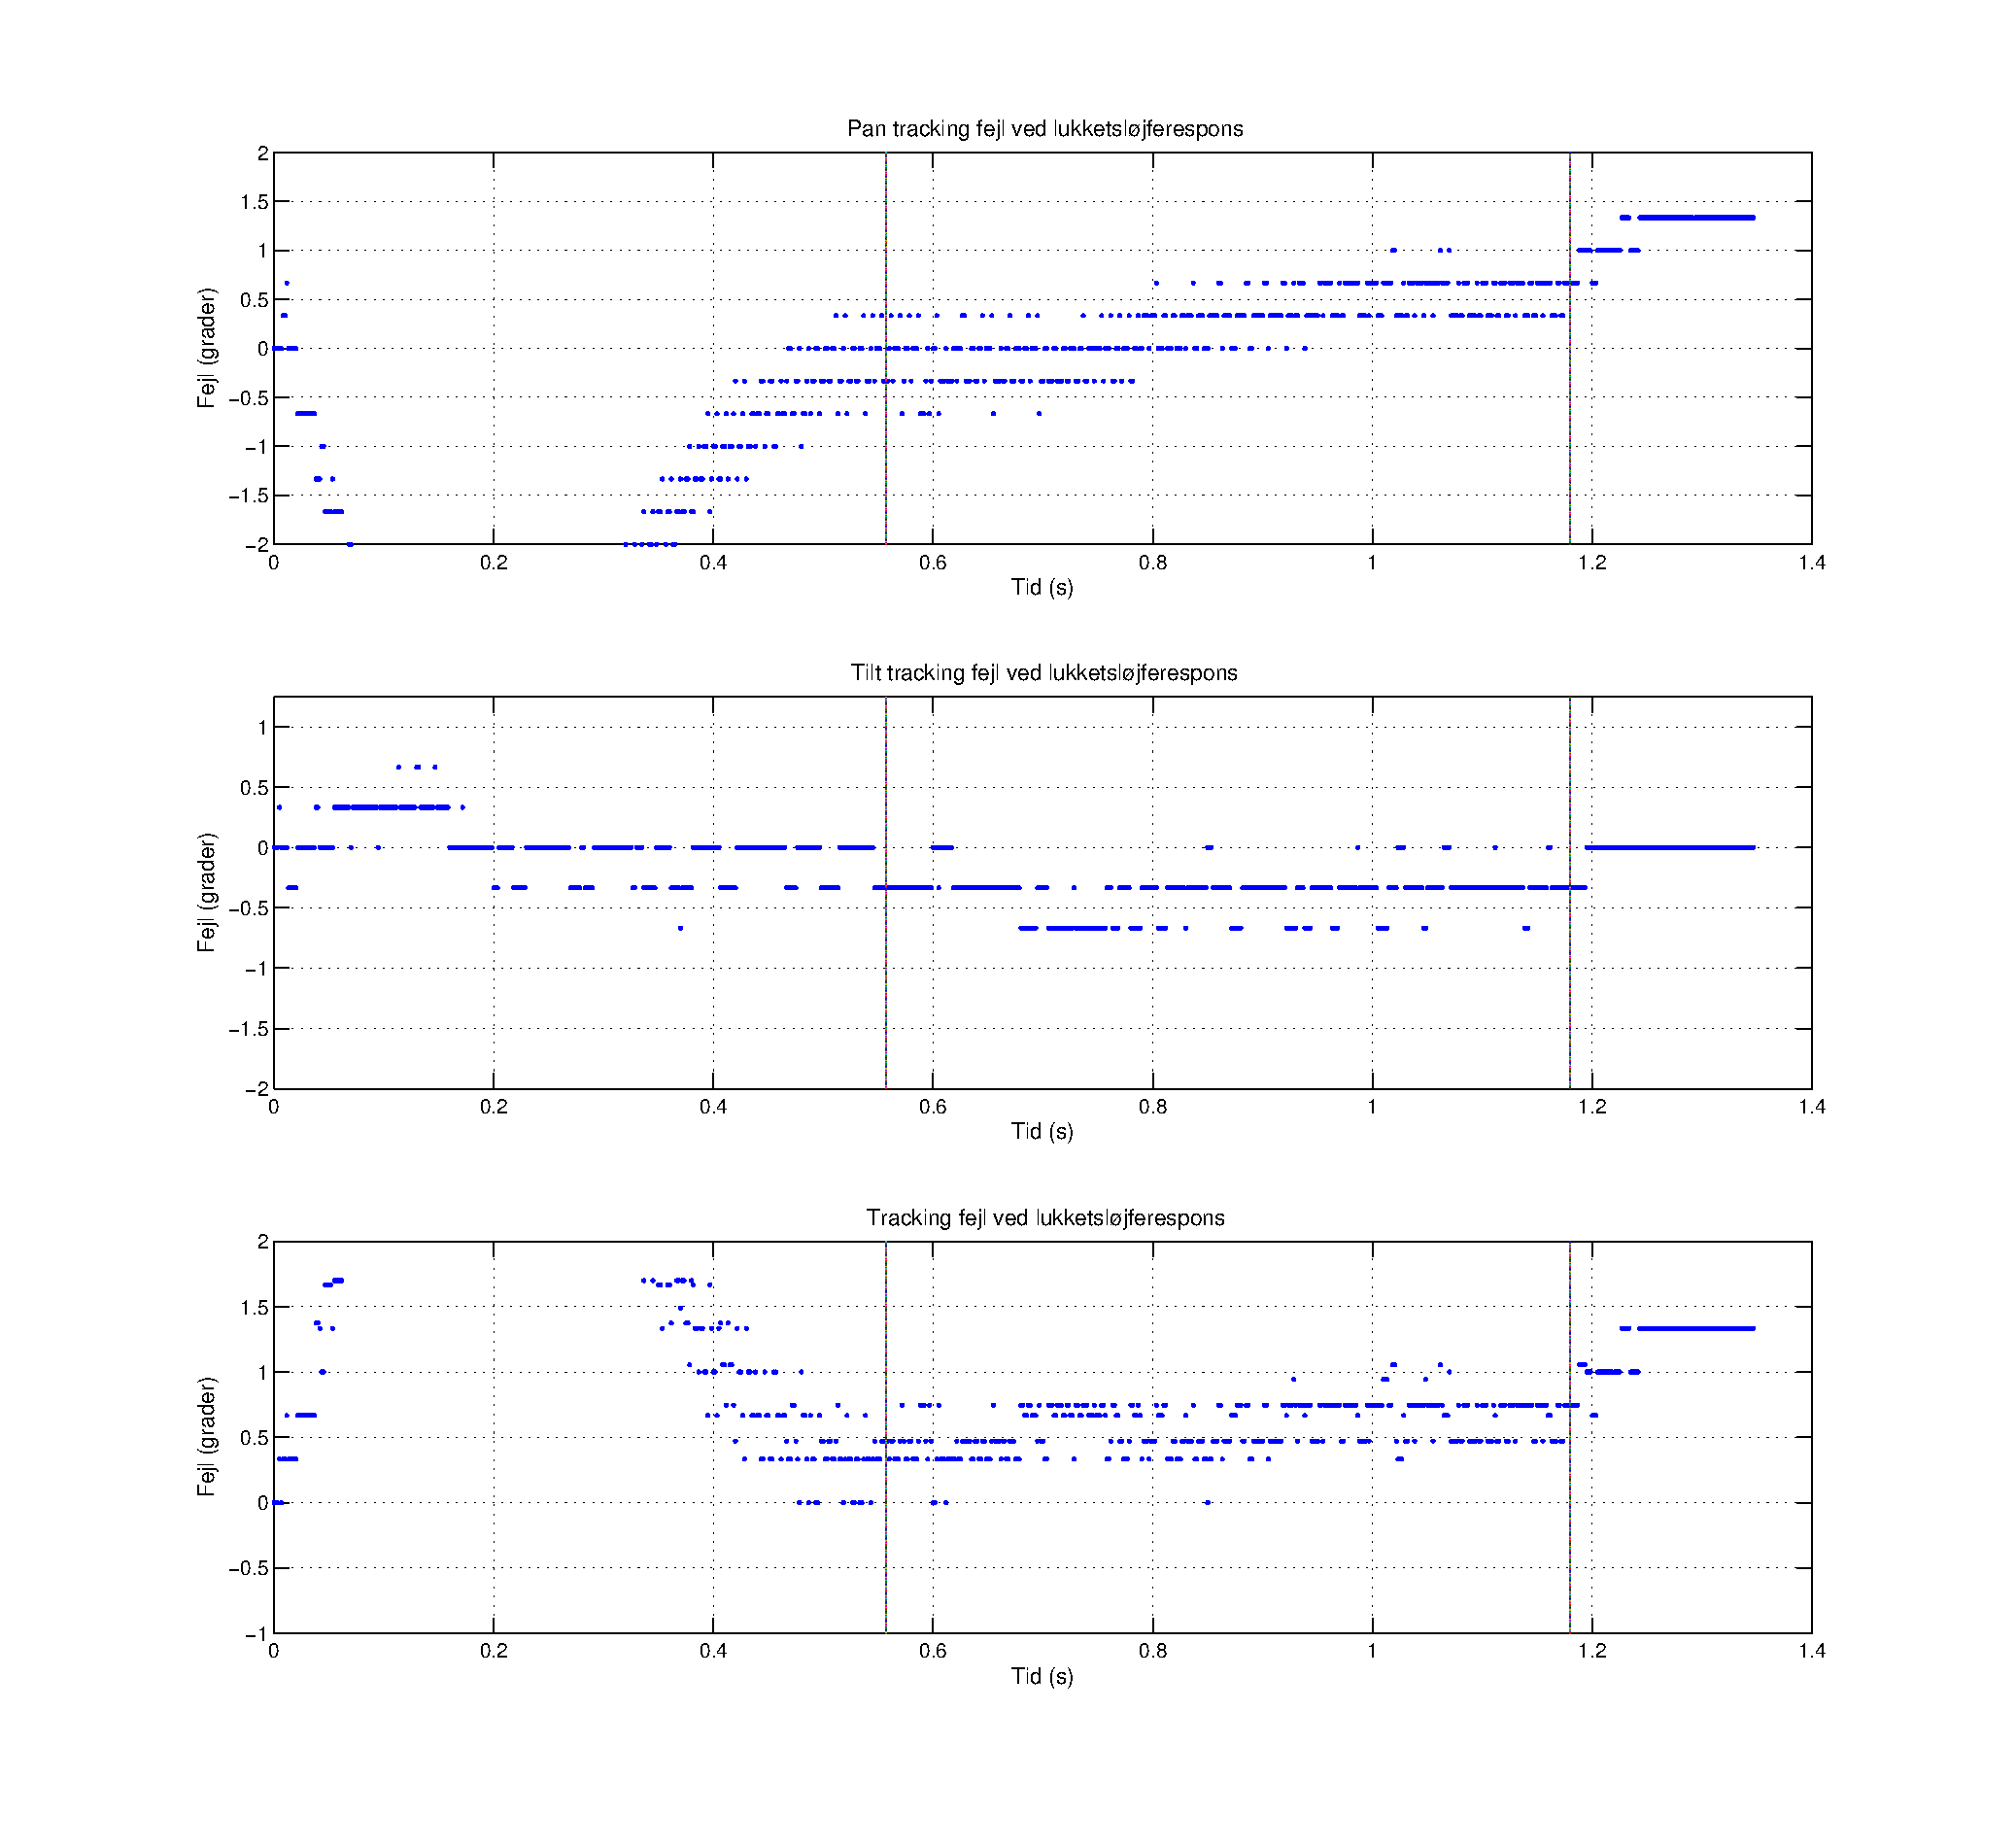
\includegraphics[width=1\textwidth]{./graphics/error_slut.eps}
%\caption[Endelig regulator koefficienter]{Tracking fejl målt i grader for hhv. pan og tilt samt den samlet tracking fejl. Testen tager udgangspunkt i koefficienterne fra  tabel \ref{tb:PID_final} og det ses at den samlet tracking fejl opfylder kravet til PTS.} 
%\label{fig:PID_final}
%\end{figure}

Det viste sig under justeringen at systemet er meget følsomt overfor slid i drivremmene mellem motorerne og Pan- og Tilt-rammerne.
Systemet kræver derfor kalibrering for at kunne fungere i praksis.

\section{Delkonlusion}
Ved Trial-\&-Error-metoden blev regulatorkoefficienterne i Simulink justeret til at give den ønskede 
tracking performance ift. et parabelinput. Pan-koefficienterne giver dårlig performance i praksis.
Ved manuel justering blev et sæt PID-regulatorkoefficienter fundet til Pan, som gav bedre performance.
Det vurderedes nødvendigt at implementere et lavpasfilter til D-leddet.
Med det implementerede filter gav de justerede regulatorkoefficienter en performance,
der ikke ved alle forsøg levede op til kravspecifikationen. Ved nogle af forsøgene viste
systemet sig at leve op til kravene om en Tracking fejl på under 1,02 \degree{} efter 0,557 [s].
Systemet er følsomt overfor slid i drivremmene.